\documentclass[hyperref=colorlinks]{beamer}
\mode<presentation>
\usetheme{iclpt}
\setbeamertemplate{navigation symbols}{}
\setbeamertemplate{headline}{
\begin{beamercolorbox}[leftskip=.2cm,rightskip=.2cm,topskip=.2cm,ht=1.1cm,dp=0.1cm,wd=\textwidth]{institute in head/foot}
  
\includegraphics[height=1cm]{icl.pdf}
  \hfill
  
\includegraphics[height=1cm]{../Pics/CMS-Color.pdf}
\end{beamercolorbox}
}
\setbeamertemplate{footline}{
\begin{beamercolorbox}[ht=.55cm,dp=0.4cm,wd=\textwidth,leftskip=.3cm]{author in head/foot}%
  \begin{minipage}[c]{5cm}%
    \usebeamerfont{author in head/foot}
    \insertshortauthor 
    \insertshorttitle
    \end{minipage}\hfill%
  \insertframenumber{} / \pageref{lastframe}
  \hfill
  \begin{minipage}{6cm}
    \hfill
  \end{minipage}
\end{beamercolorbox}%
}

\usepackage{color}
\usepackage{tabularx,colortbl}
\usepackage{graphicx}
\usepackage{pdfpages}
\usepackage{feynmp}
\usepackage{multirow}
\DeclareGraphicsRule{*}{mps}{*}{}

\title{\vspace{-0.2cm} VBF Higgs to Invisible Trigger Efficiencies}
%\subtitle{This result: HIG-15-012 \\ Contributing analyses: HIG-13-030, HIG-14-038, EXO-12-055}
\author[P. Dunne]{\underline{P. Dunne} on behalf of the H$\rightarrow$invisible analysis group}
\titlegraphic{
  \vspace{-0.7cm}
  %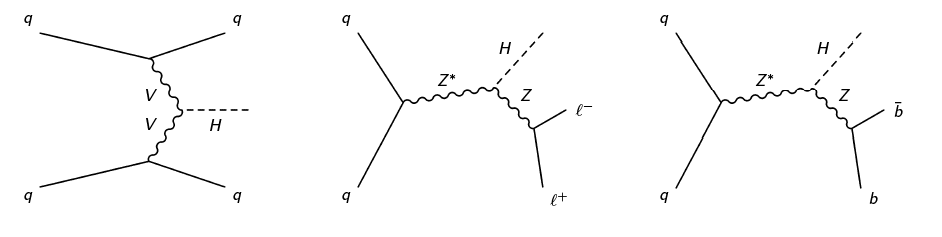
\includegraphics[width=\textwidth]{TalkPics/invcomb021213/feyndiags}
%% \begin{fmfgraph*}(100,70)
%%         \fmfleft{i1,i2}
%%         \fmfright{o1,o2,o3}
%%         \fmf{fermion}{i1,v1,o1}
%%         \fmf{fermion}{i2,v2,o3}
%%         \fmf{phantom,tension=4/5}{v1,v2}
%%         \fmffreeze
%%         \fmf{photon,label=$W,,Z$}{v1,v3}
%%         \fmf{photon,label=$W,,Z$}{v2,v3}
%%         \fmf{dashes}{v3,o2}
%%         \fmflabel{$q$}{i1}
%%         \fmflabel{$q$}{i2}
%%         \fmflabel{$q$}{o1}
%%         \fmflabel{$q$}{o3}
%%         \fmflabel{$H$}{o2}
%%       \end{fmfgraph*}
}
\date{}
\begin{document}
\begin{fmffile}{hexotrig261015feyndiags}

%TITLE PAGE
\section{Title}
\begin{frame}
  \titlepage
  
\end{frame}

%!!CLOSURE TEST STATEMENT PU jet ID
%OUTLINE
\begin{frame}
  \frametitle{VBF - Higgs to Invisible in Run II}
  \scriptsize
  \vspace{-.2cm}
    \begin{block}{}
      \begin{itemize}
      \item At the end of run 1 significant BSM Higgs properties are not excluded:
      \item[-] Direct CMS observed (expected) limit 36 (30)\% 
      \item[-] Indirect limit from ATLAS+CMS on BR$_{BSM}\sim 35\%$
      \item Most sensitive VBF channel is still statistically limited
      \item[-] Need as much data in run 2 as possible
      \end{itemize}
    \end{block}
  
  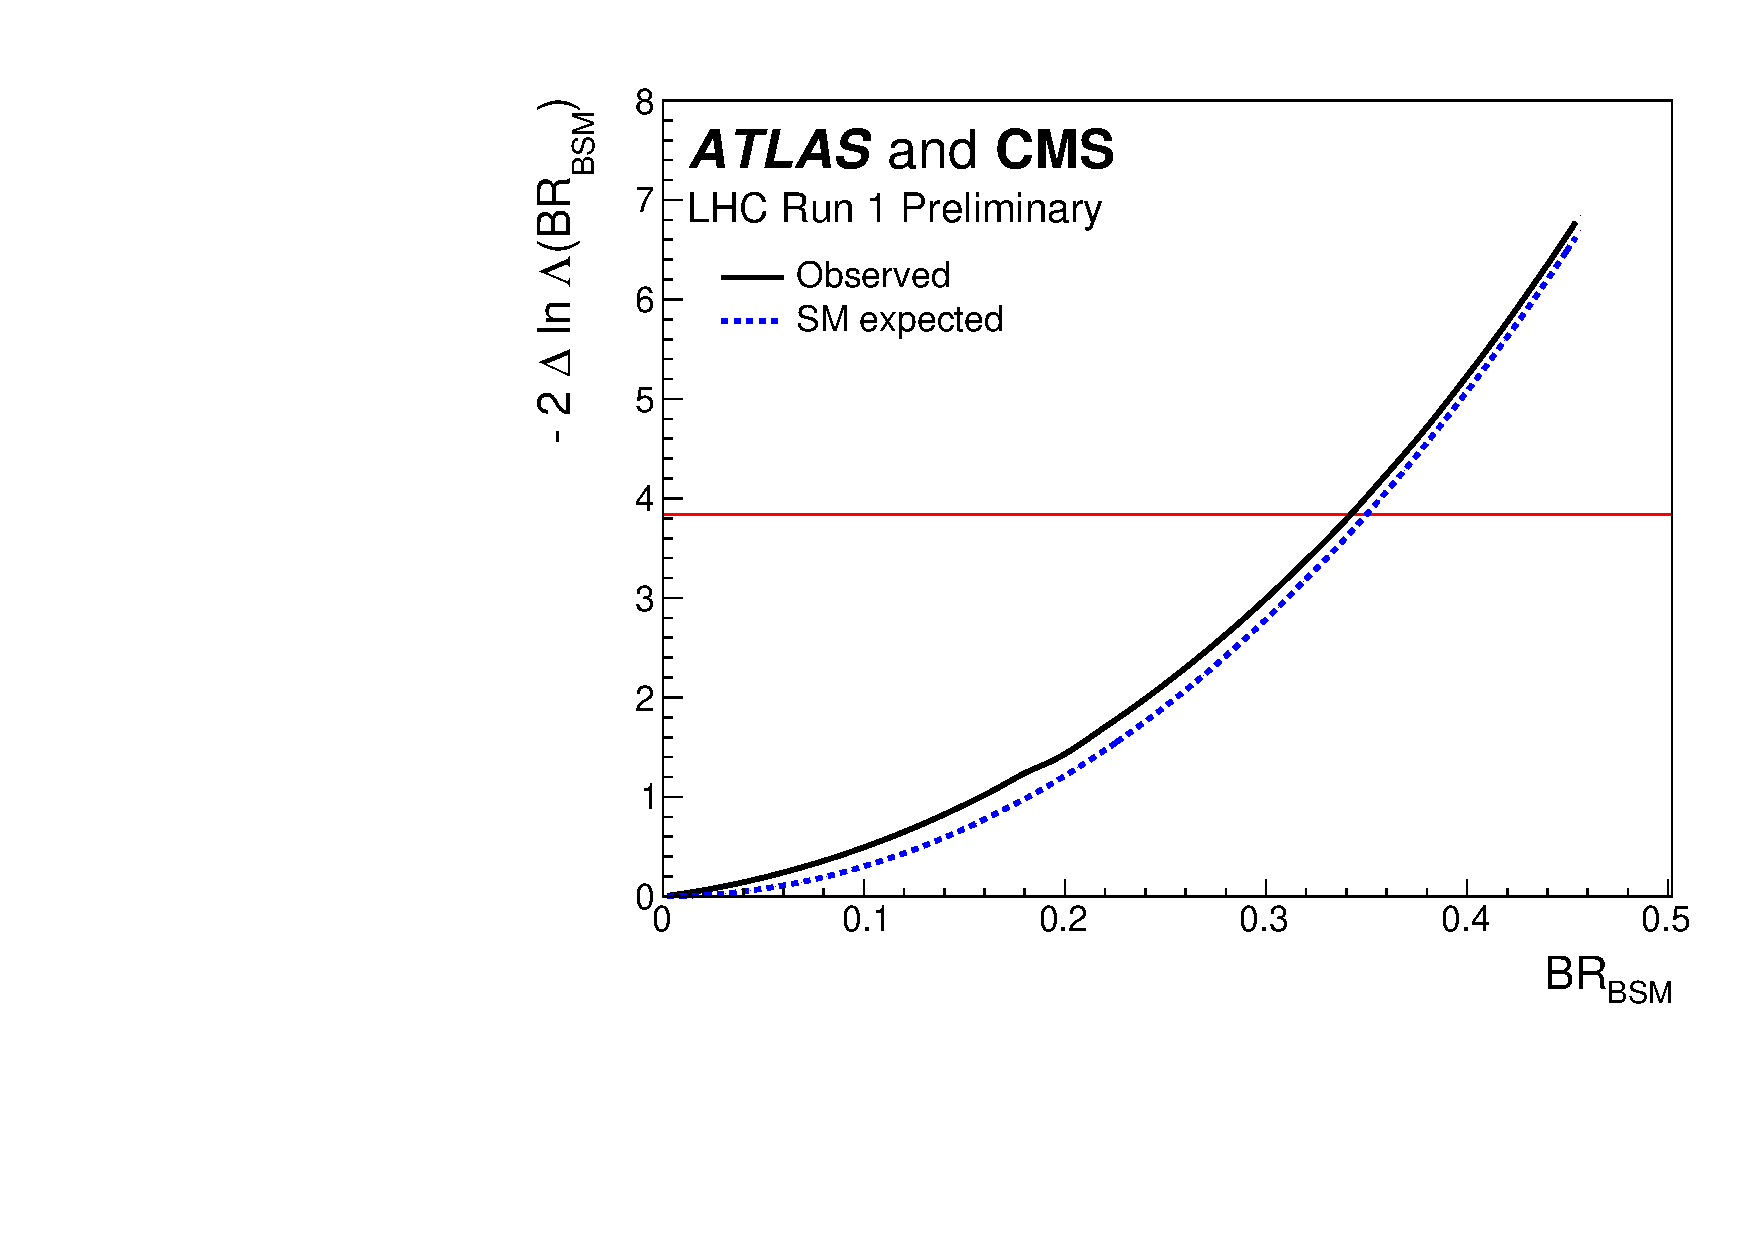
\includegraphics[height=.55\textheight]{TalkPics/iccms300915/CMS-PAS-HIG-15-002_Figure_015.pdf}
  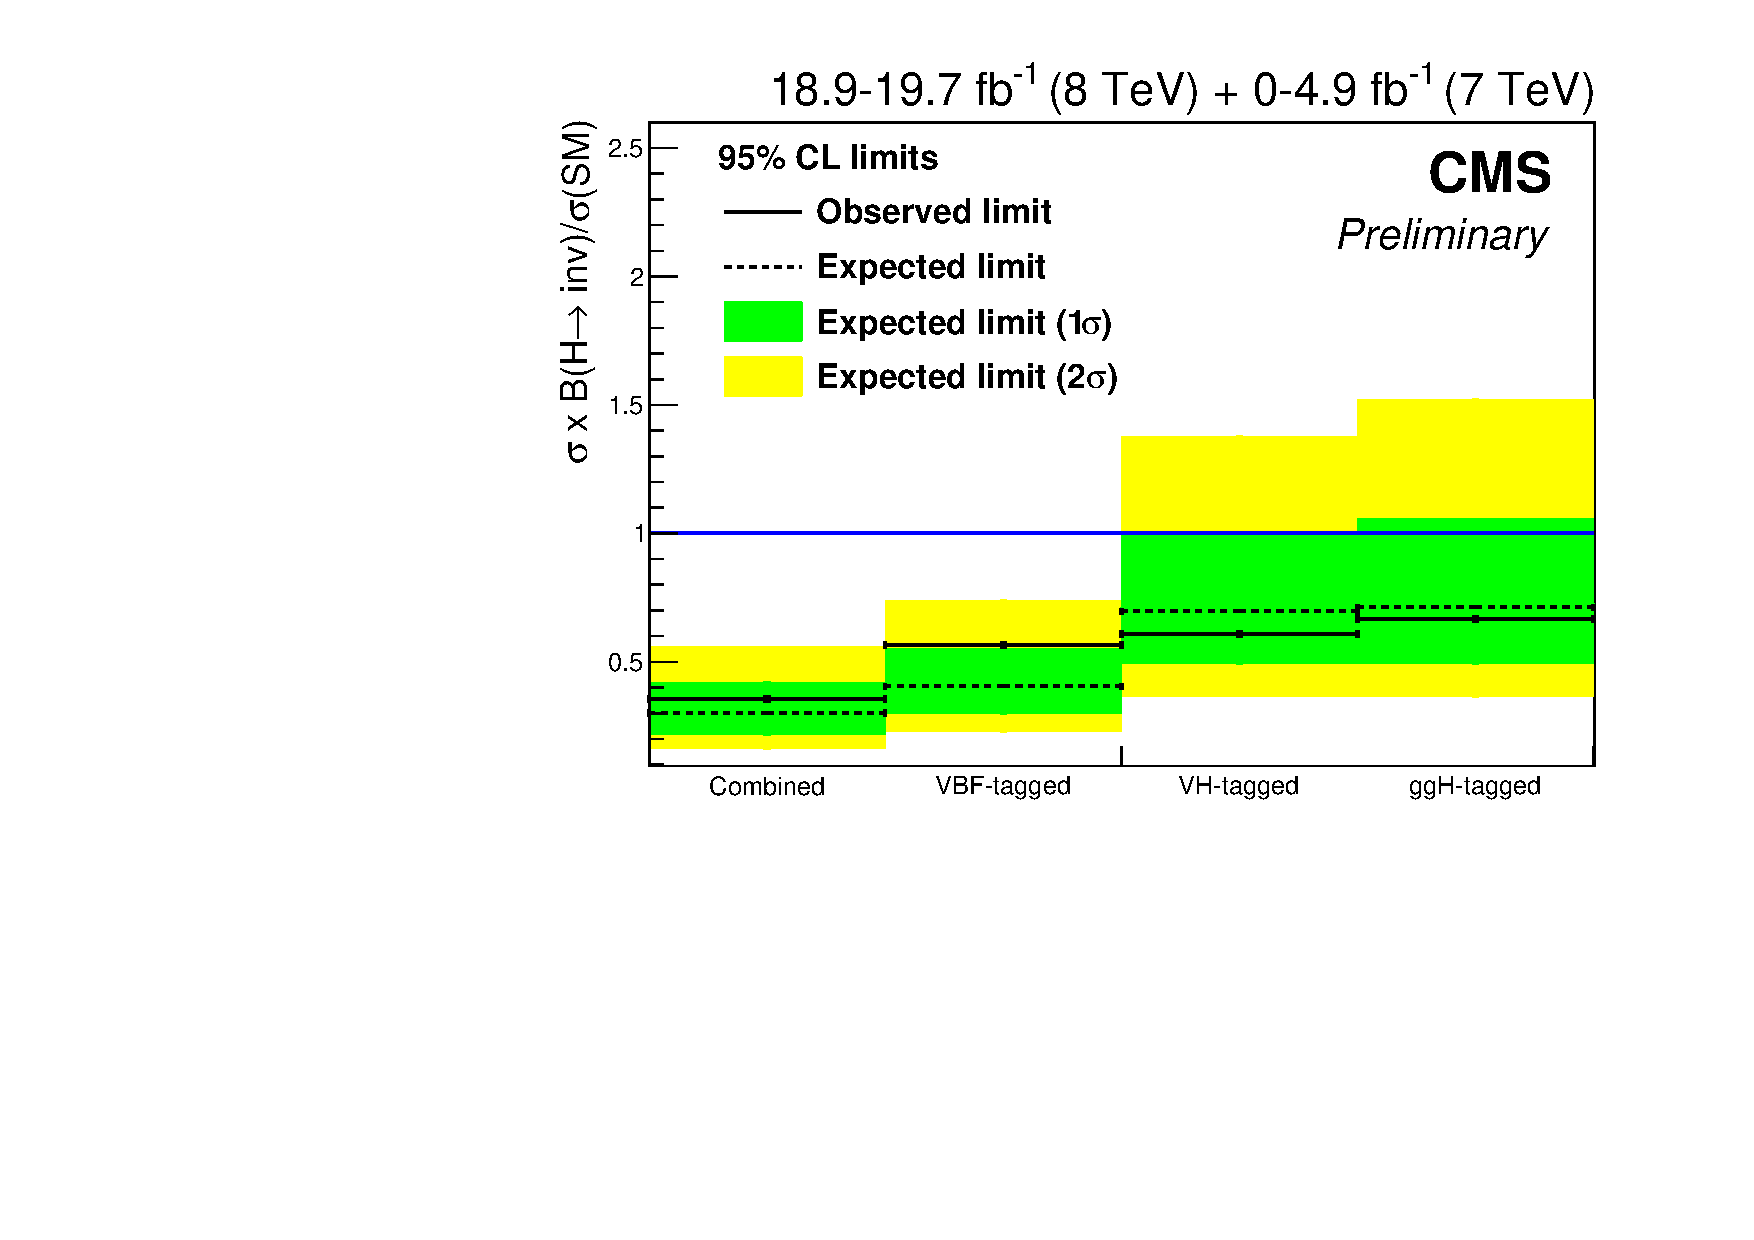
\includegraphics[height=.55\textheight]{TalkPics/studentseminar221015/hig15012figures/channellimit.pdf}
\end{frame}

\begin{frame}
  \frametitle{Triggers and Dataset}
  \scriptsize
  \vspace{-.2cm}
  \begin{block}{Triggers}
    \begin{itemize}
    \item We have two triggers runnning for VBF Higgs to invisible:
    \item[-] Signal trigger: unprescaled HLT\_DiPFJet40\_DEta3p5\_MJJ600\_PFMETNoMu140
    \item[-] Prescaled HLT\_DiPFJet40\_DEta3p5\_MJJ600\_PFMETNoMu80
    \item Will show efficiencies for signal trigger today
    \end{itemize}
  \end{block}
  \begin{block}{Dataset used for efficiency measurement}
    \begin{itemize}
    \item Use SingleMuon dataset to measure efficiency
    \item[-] We have 1280 pb$^{-1}$ processed
    \item We are using the latest 74X\_dataRun2\_Prompt\_v4 jet energy corections
    \item We are using the latest MET filter recipes
    \item[-] CSC filter is due to be replaced with an event list to veto although this is not yet available
    \item Cuts for efficiency denominator chosen where trigger is 90\% efficient
    \end{itemize}
  \end{block}
\end{frame}

\begin{frame}
  \frametitle{Trigger Efficiencies}
  \scriptsize
  \begin{block}{}
    \begin{itemize}
    \item Denominator is all events in SingleMuon passing:
    \item[-] METnoMu$>300$ GeV, DiPFJet$>80$ GeV, $\Delta\eta_{jj}>3.6$, $M_{jj}>$600
    \item Cut on variable shown is not applied
    \end{itemize}
  \end{block}
  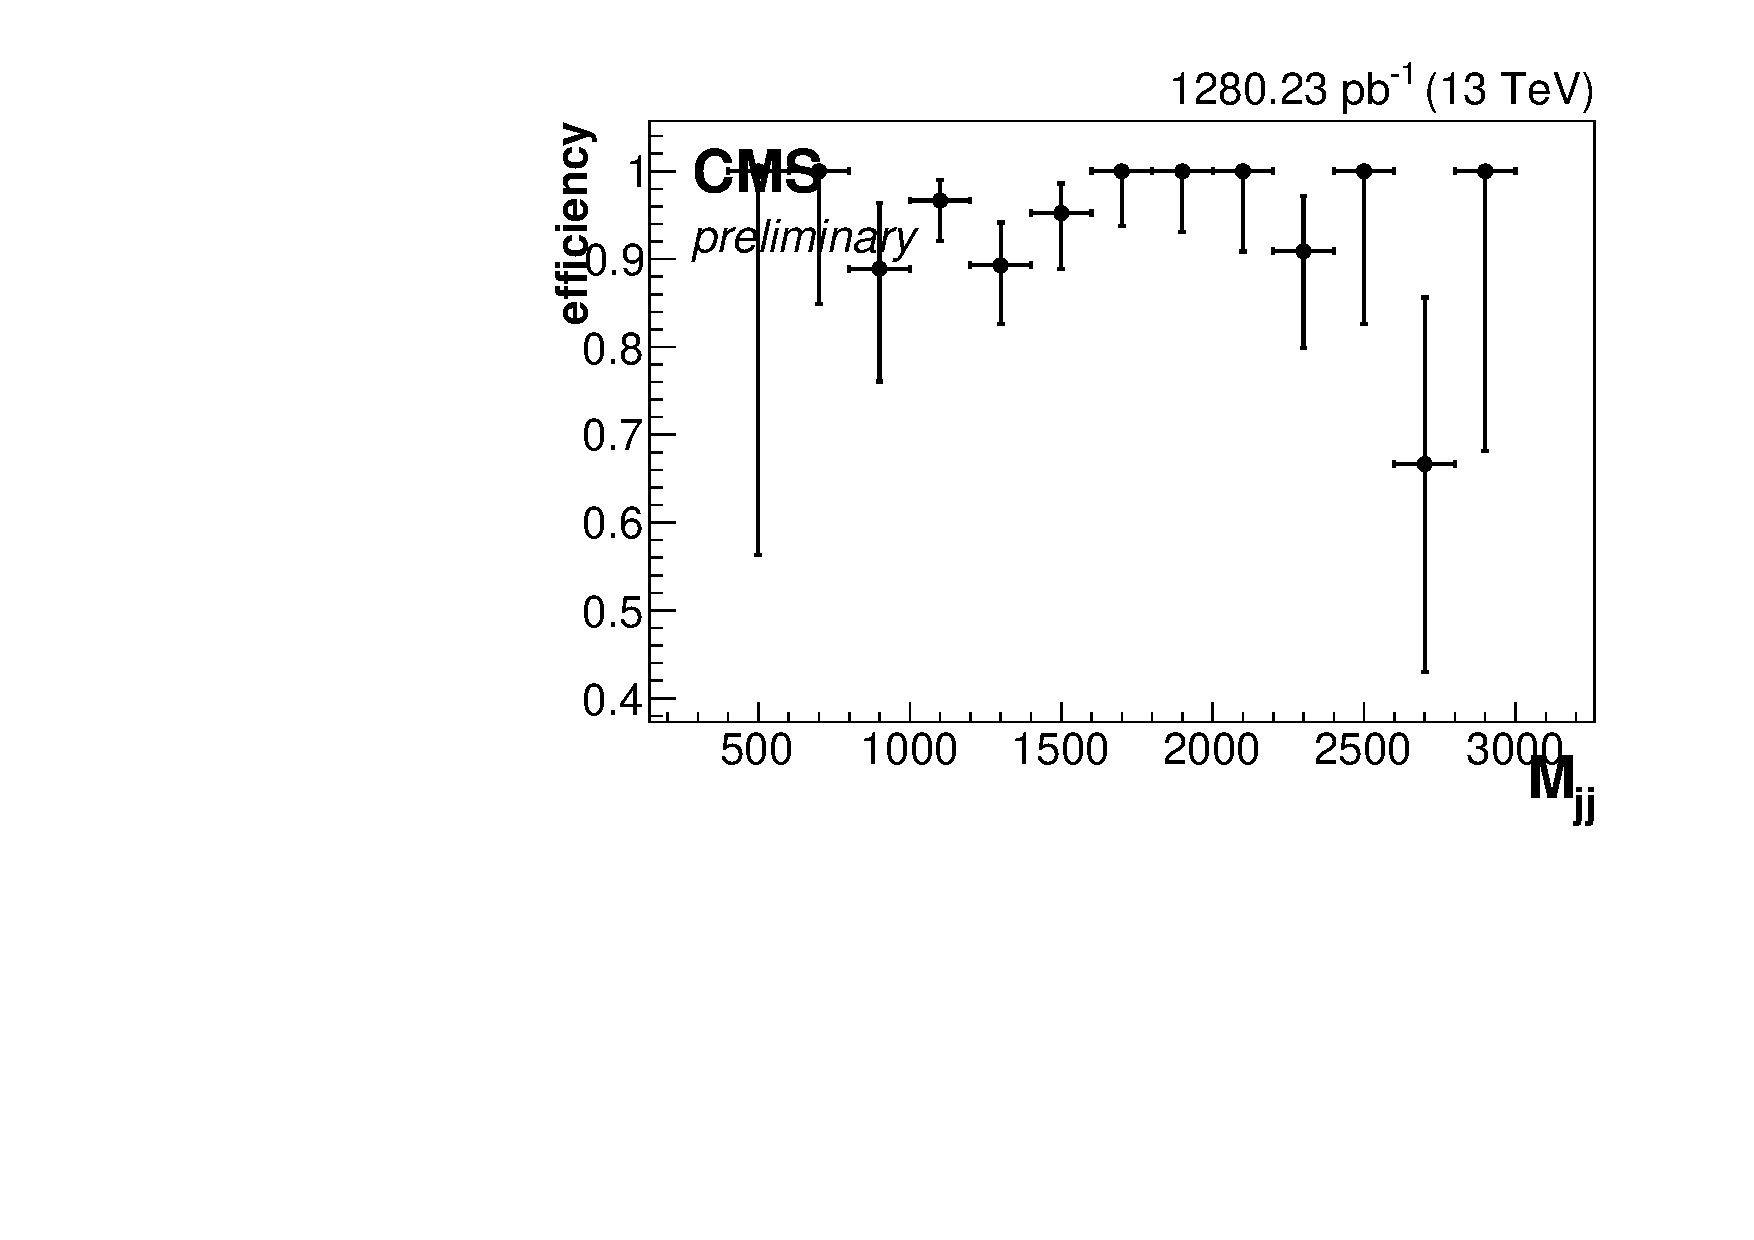
\includegraphics[width=.5\textwidth]{TalkPics/hexotrig261015/output_2015Dtrigeff_261015/nunu_dijet_M.pdf}
  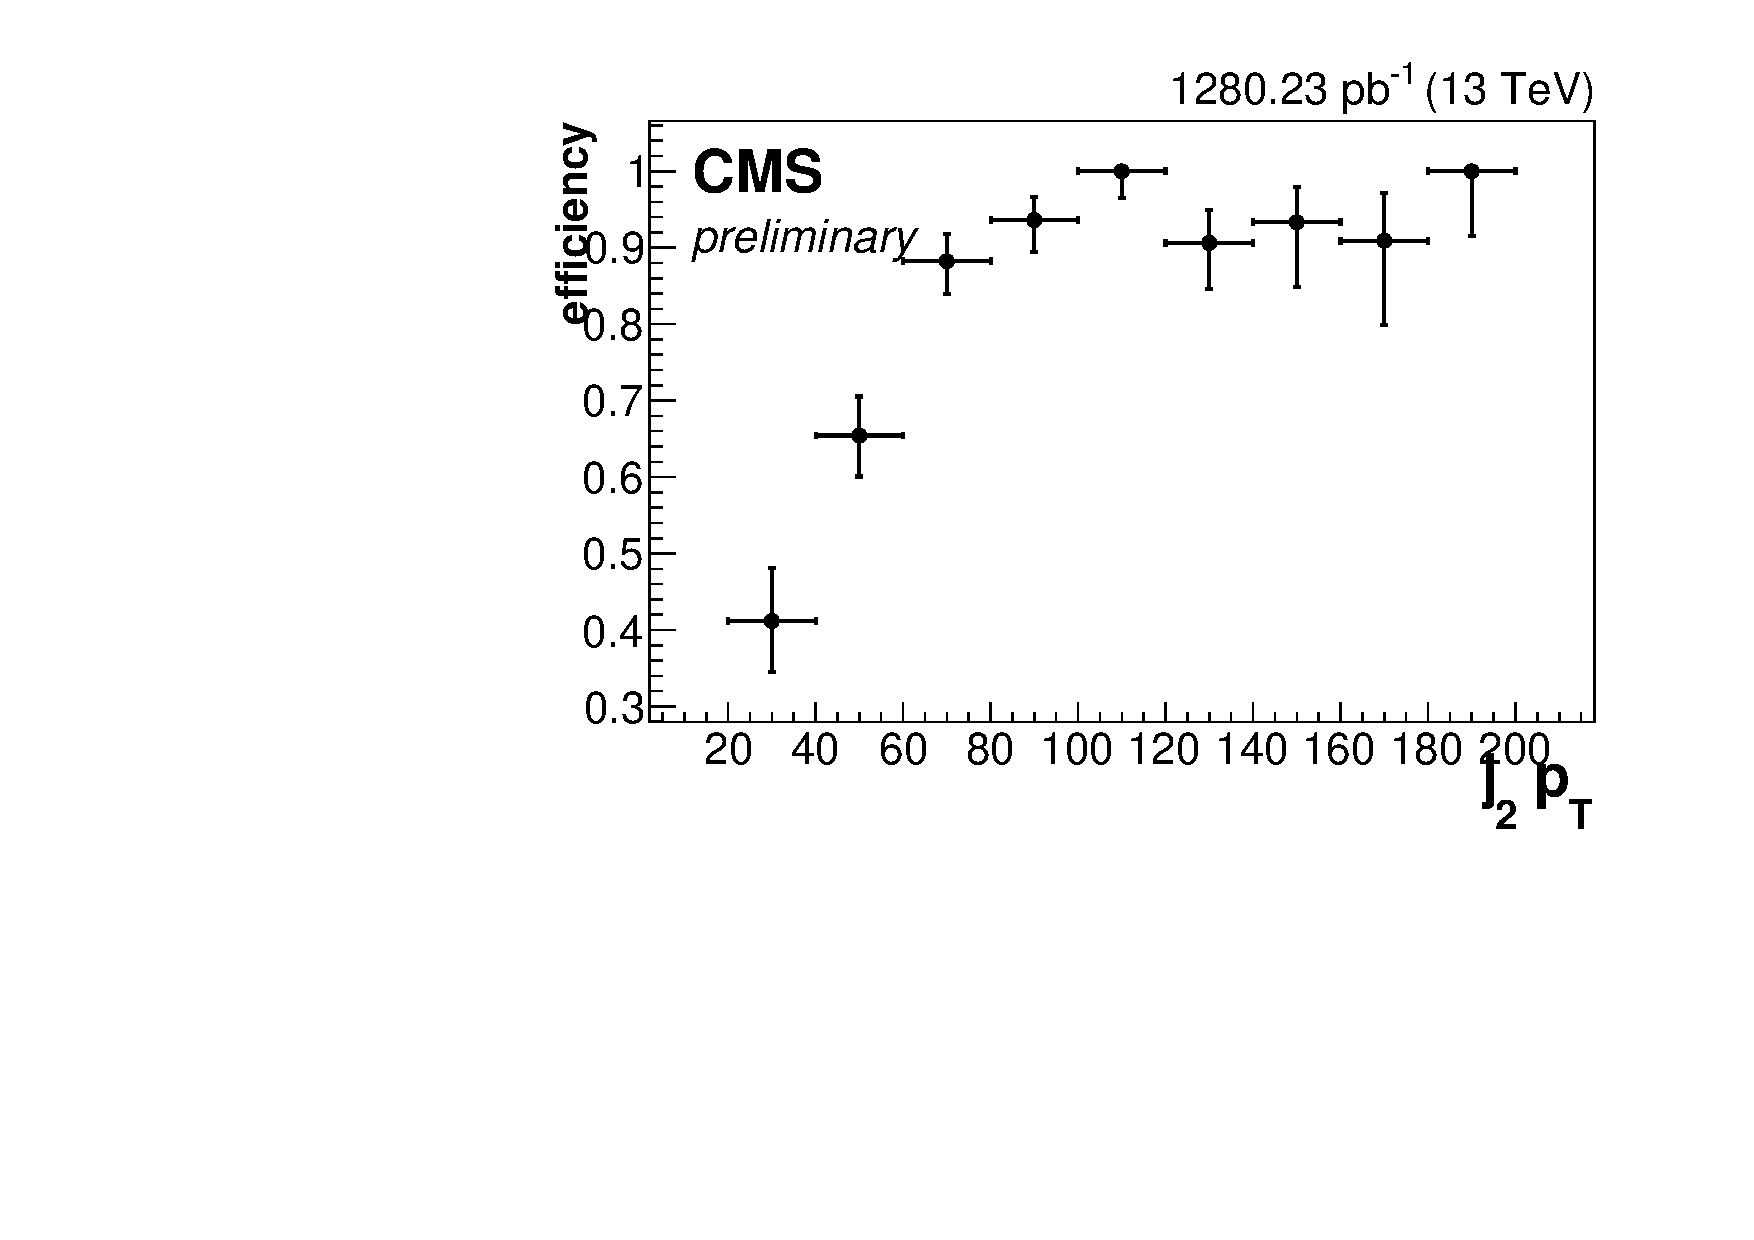
\includegraphics[width=.5\textwidth]{TalkPics/hexotrig261015/output_2015Dtrigeff_261015/nunu_jet2_pt.pdf}
\end{frame}

\begin{frame}
  \frametitle{Trigger Efficiencies}
  \scriptsize
  \begin{block}{}
    \begin{itemize}
    \item Denominator is all events in SingleMuon passing:
    \item[-] METnoMu$>300$ GeV, DiPFJet$>80$ GeV, $\Delta\eta_{jj}>3.6$, $M_{jj}>$600
    \item Cut on variable shown is not applied
    \end{itemize}
  \end{block}
  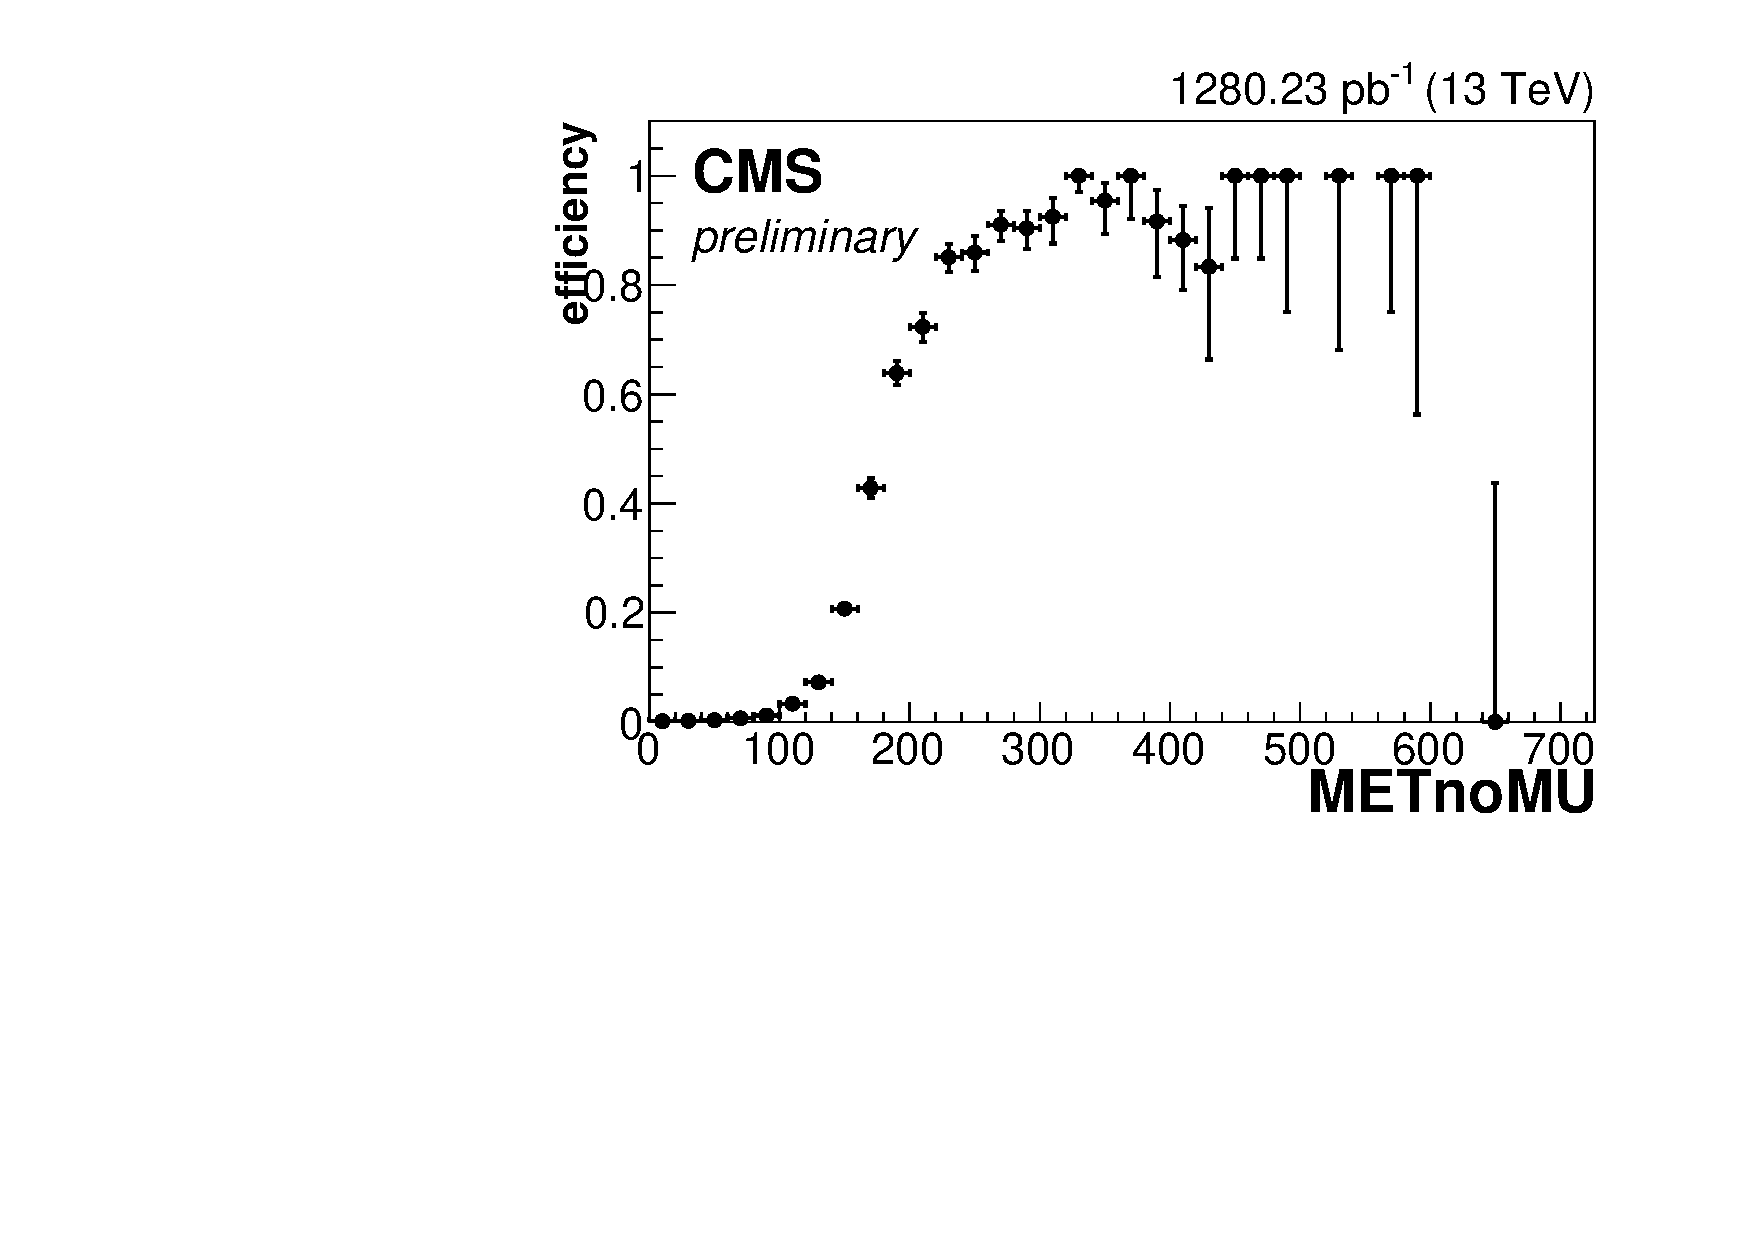
\includegraphics[width=.5\textwidth]{TalkPics/hexotrig261015/output_2015Dtrigeff_261015/nunu_metnomuons.pdf}
  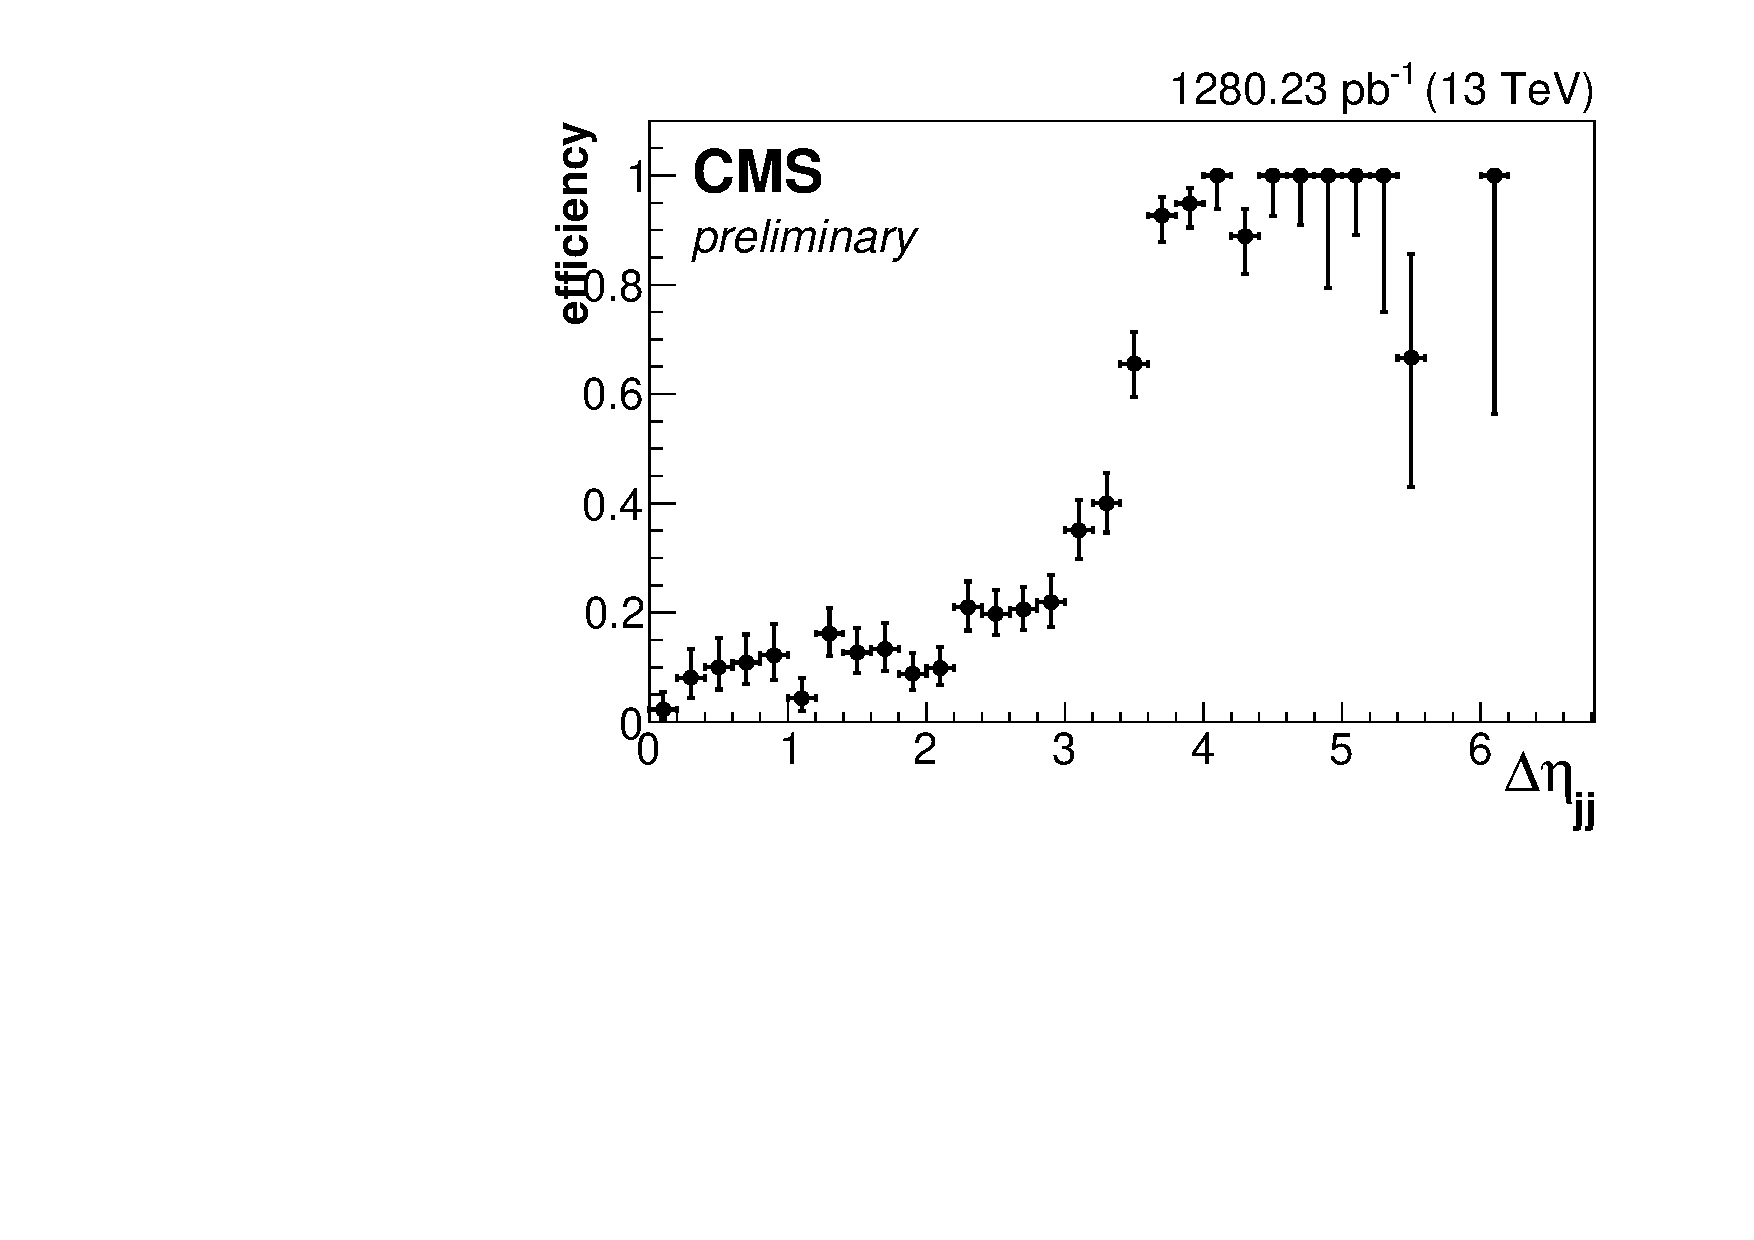
\includegraphics[width=.5\textwidth]{TalkPics/hexotrig261015/output_2015Dtrigeff_261015/nunu_dijet_deta.pdf}
\end{frame}

\begin{frame}
  \frametitle{Summary}
  \label{lastframe}
  \begin{block}{}
    \begin{itemize}
    \item Trigger efficiencies from 25ns data shown
    \item Possible dips in efficiency above turn on in MET and jet 2 pt
    \item[-] Need investigating and monitoring as statistics increase
    \item MET and jet $p_{T}$ turn ons are very high
    \item We will continue to update these plots as new luminosity and recipes become available
    \end{itemize}
  \end{block}
  \centering
\end{frame}

%UPDATED BACKUP
\begin{frame}
  \frametitle{Backup}
\end{frame}

\begin{frame}
\end{frame}

\end{fmffile}
\end{document}
